\documentclass[11pt]{article}
\usepackage[margin=0.78in]{geometry}
\usepackage{amsmath,amssymb}
\usepackage{booktabs}
\usepackage{graphicx}
\usepackage{xcolor}
\usepackage{hyperref}
\usepackage{tikz}
\usetikzlibrary{arrows.meta,positioning,shapes.geometric,fit,calc,matrix}
\hypersetup{colorlinks=true,linkcolor=blue!45!black,urlcolor=blue!55!black}
\setlength{\parindent}{0pt}
\setlength{\parskip}{0.55em}
\newcommand{\status}[1]{\textbf{Status: #1}}
\newcommand{\artifact}[1]{\texttt{\detokenize{#1}}}
\newcommand{\schematicnote}{\textit{This is a schematic, not evidence.}}
\newcommand{\lookat}{\textbf{What to look at.} }
\newcommand{\caveat}{\textbf{Caveat.} }
\newcommand{\bottomline}{\textbf{Bottom line.} }
\newcommand{\codeword}[1]{\texttt{#1}}
\definecolor{trusted}{HTML}{1B9E77}
\definecolor{broken}{HTML}{D73027}
\definecolor{caution}{HTML}{E6AB02}
\definecolor{muted}{HTML}{777777}
\definecolor{gpu}{HTML}{7570B3}

\title{Why the GOTHAM PDF Files Broke\\\large A shared-buffer bug with a very specific fingerprint}
\author{GOTHAM PDF reconstruction notes}
\date{June 2026}

\begin{document}
\maketitle

\status{Strongly supported root cause. A same-state broken-line/fixed-line
AthenaK reproduction has not yet been run.}

\section{What we are trying to explain}

Fourteen multidimensional PDF stream definitions were used during the five
GOTHAM simulations. The corruption summary reports that, at the checked latest
snapshots, twelve are unusable for radial or angular diagnostics. One,
\codeword{output29}, keeps a trustworthy angle-integrated radial profile but
not its angular distribution. One, \codeword{output31}, remains useful. The
attempted full archive audit failed before writing its final CSV, so the
archive-wide scope is not independently preserved as a completed artifact.

That mixed outcome is the question. A vague ``the PDFs are corrupted'' story
is not enough. We need a mechanism that predicts \emph{which} axes fail,
\emph{which} marginals survive, and why total weight can remain nearly right
while the joint distribution is badly wrong.

\section{The simple picture}

Here is the simple version. AthenaK computed several derived coordinates into
one shared array. The \codeword{coord\_abscostheta} routine resized that array
after earlier coordinates had already been written. In Kokkos,
\codeword{realloc} does not promise to preserve the old contents. The new angle
was written. Earlier rows, including radius in the affected orderings, became
unsafe. In the affected archive, unsafe radius behaves like zero and lands in
radial underflow; unsafe \codeword{coord\_abscostheta} behaves like zero and
lands in its first interior bin.

The simulation state was fine. The histogram formulas were mostly fine. The
temporary coordinate workspace was not.

\section{The cartoon version}

\begin{figure}[ht]
\centering
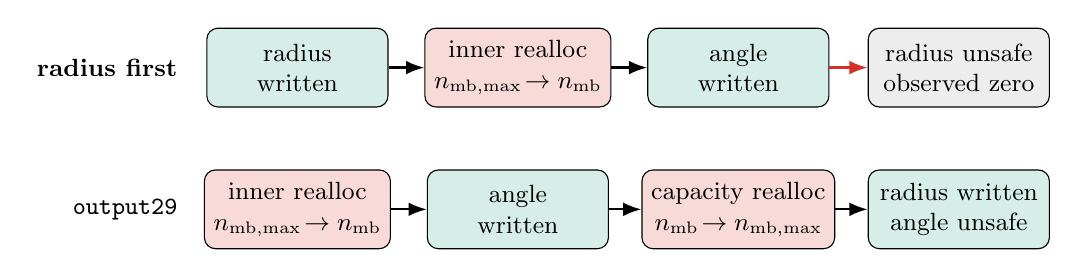
\begin{tikzpicture}[>=Latex,
  box/.style={draw,rounded corners,minimum width=23mm,minimum height=10mm,align=center,font=\small},
  good/.style={box,fill=trusted!18},
  bad/.style={box,fill=broken!18},
  blank/.style={box,fill=black!7}]
\node[anchor=east,font=\bfseries\small] at (-0.2,0) {radius first};
\node[good] (r1) at (1.2,0) {radius\\written};
\node[bad] (ri) at (4.0,0) {inner realloc\\$n_{\rm mb,max}\!\to n_{\rm mb}$};
\node[good] (a1) at (6.8,0) {angle\\written};
\node[blank] (rlost) at (9.6,0) {radius unsafe\\observed zero};
\draw[->,thick] (r1)--(ri);
\draw[->,thick] (ri)--(a1);
\draw[->,thick,broken] (a1)--(rlost);

\node[anchor=east,font=\bfseries\small] at (-0.2,-1.8) {\codeword{output29}};
\node[bad] (ai) at (1.2,-1.8) {inner realloc\\$n_{\rm mb,max}\!\to n_{\rm mb}$};
\node[good] (a2) at (4.0,-1.8) {angle\\written};
\node[bad] (rc) at (6.8,-1.8) {capacity realloc\\$n_{\rm mb}\!\to n_{\rm mb,max}$};
\node[good] (r2) at (9.6,-1.8) {radius written\\angle unsafe};
\draw[->,thick] (ai)--(a2);
\draw[->,thick] (a2)--(rc);
\draw[->,thick] (rc)--(r2);
\end{tikzpicture}
\caption{The bad angle call causes one destructive reallocation in
radius-first products and triggers a second capacity reallocation before
radius in \codeword{output29}. The coordinate written last survives.
\schematicnote}
\end{figure}

Read this left to right. Before the angle routine runs, the shared workspace
already contains rows written by earlier coordinate routines. The inner
\codeword{realloc} replaces that storage, shrinks its first extent from
\(n_{\rm mb,max}\) to \(n_{\rm mb}\), and the angle routine fills back only its
own row.

Now comes the part that explains \codeword{output29}. Its next coordinate is
radius. At the start of that call, the common capacity check sees
\(n_{\rm mb}<n_{\rm mb,max}\), reallocates the workspace back to
\(n_{\rm mb,max}\), invalidates the angle row, and then writes radius. So the
two orders fail differently:
\[
\begin{array}{ll}
\text{radius first:} & r\ \longrightarrow\ \text{inner realloc}\ \longrightarrow\
|\cos\theta| \quad \Rightarrow\quad r\ \text{lost},\\
\text{angle first:} & |\cos\theta|\ \longrightarrow\ \text{capacity realloc}\
\longrightarrow r \quad \Rightarrow\quad |\cos\theta|\ \text{lost}.
\end{array}
\]

The annoying part is that the file writer can still count every cell. It just
counts cells using a coordinate that has been replaced by zeros. So a total can
look sensible while a coordinate axis has collapsed.

\section{The more precise version}

For a PDF product \(p\), each cell \(c\) contributes to one flattened bin:
\[
H_p(b) = \sum_c \Delta V_c\,w_p(c)\,
  \mathbf{1}\!\left[B_p(\boldsymbol{q}_c)=b\right].
\]
The bug changes the coordinate vector \(\boldsymbol{q}_c\) used by the bin map
\(B_p\). For this fourteen-product catalog, the final weight rows survive:
mass and volume live outside the shared coordinate workspace, while
\codeword{mdot\_sph} and \codeword{edot\_sph} are computed after the destructive
calls. That distinction predicts the observed split:
\begin{itemize}
  \item totals can remain correct because the same weights are accumulated;
  \item a marginal over the coordinate written last can survive;
  \item the full joint distribution fails where the erased coordinate chooses
        the wrong bins.
\end{itemize}

The source history gives us an unusually clean before-and-after. Commit
\codeword{ec009a27} changed the guarded allocation into an unconditional
allocation inside \codeword{coord\_abscostheta}; commit \codeword{db953863}
removed it. The shared array is already sized near the beginning of
\codeword{ComputeDerivedVariable()}. Full hashes are recorded in the
traceability notes.

\section{What this idea predicts}

A root-cause story is only useful if it gets the exceptions right. This one
has four places where it could have failed.

\begin{tabular}{p{0.30\linewidth}p{0.31\linewidth}p{0.28\linewidth}}
\toprule
Prediction & Diagnostic & Existing result \\
\midrule
Radius-first streams collapse into radius underflow &
Streaming sparse-shard radius audit &
Reported at checked latest snapshots across all five simulations; completed
machine-readable audit artifact missing. \\
\codeword{output29} keeps its radial marginal but loses angle &
Compare rebuilt and archived full 2D distributions and radial marginals &
Full \(E_{\rm L1}=1.92\); radial-marginal \(E_{\rm L1}=1.60\times10^{-11}\). \\
\codeword{output31} stays intact because it does not use
\codeword{coord\_abscostheta} &
Compare matched eight-shard rebuilt and archived 4D controls &
Matched eight-shard full-4D \(E_{\rm L1}=3.87\times10^{-7}\). \\
Weights remain counted even when coordinates are wrong &
Compare signed totals &
Control totals agree at roughly \(10^{-12}\) normalized error. \\
\bottomrule
\end{tabular}

\section{What the evidence actually shows}

\begin{figure}[p]
\centering
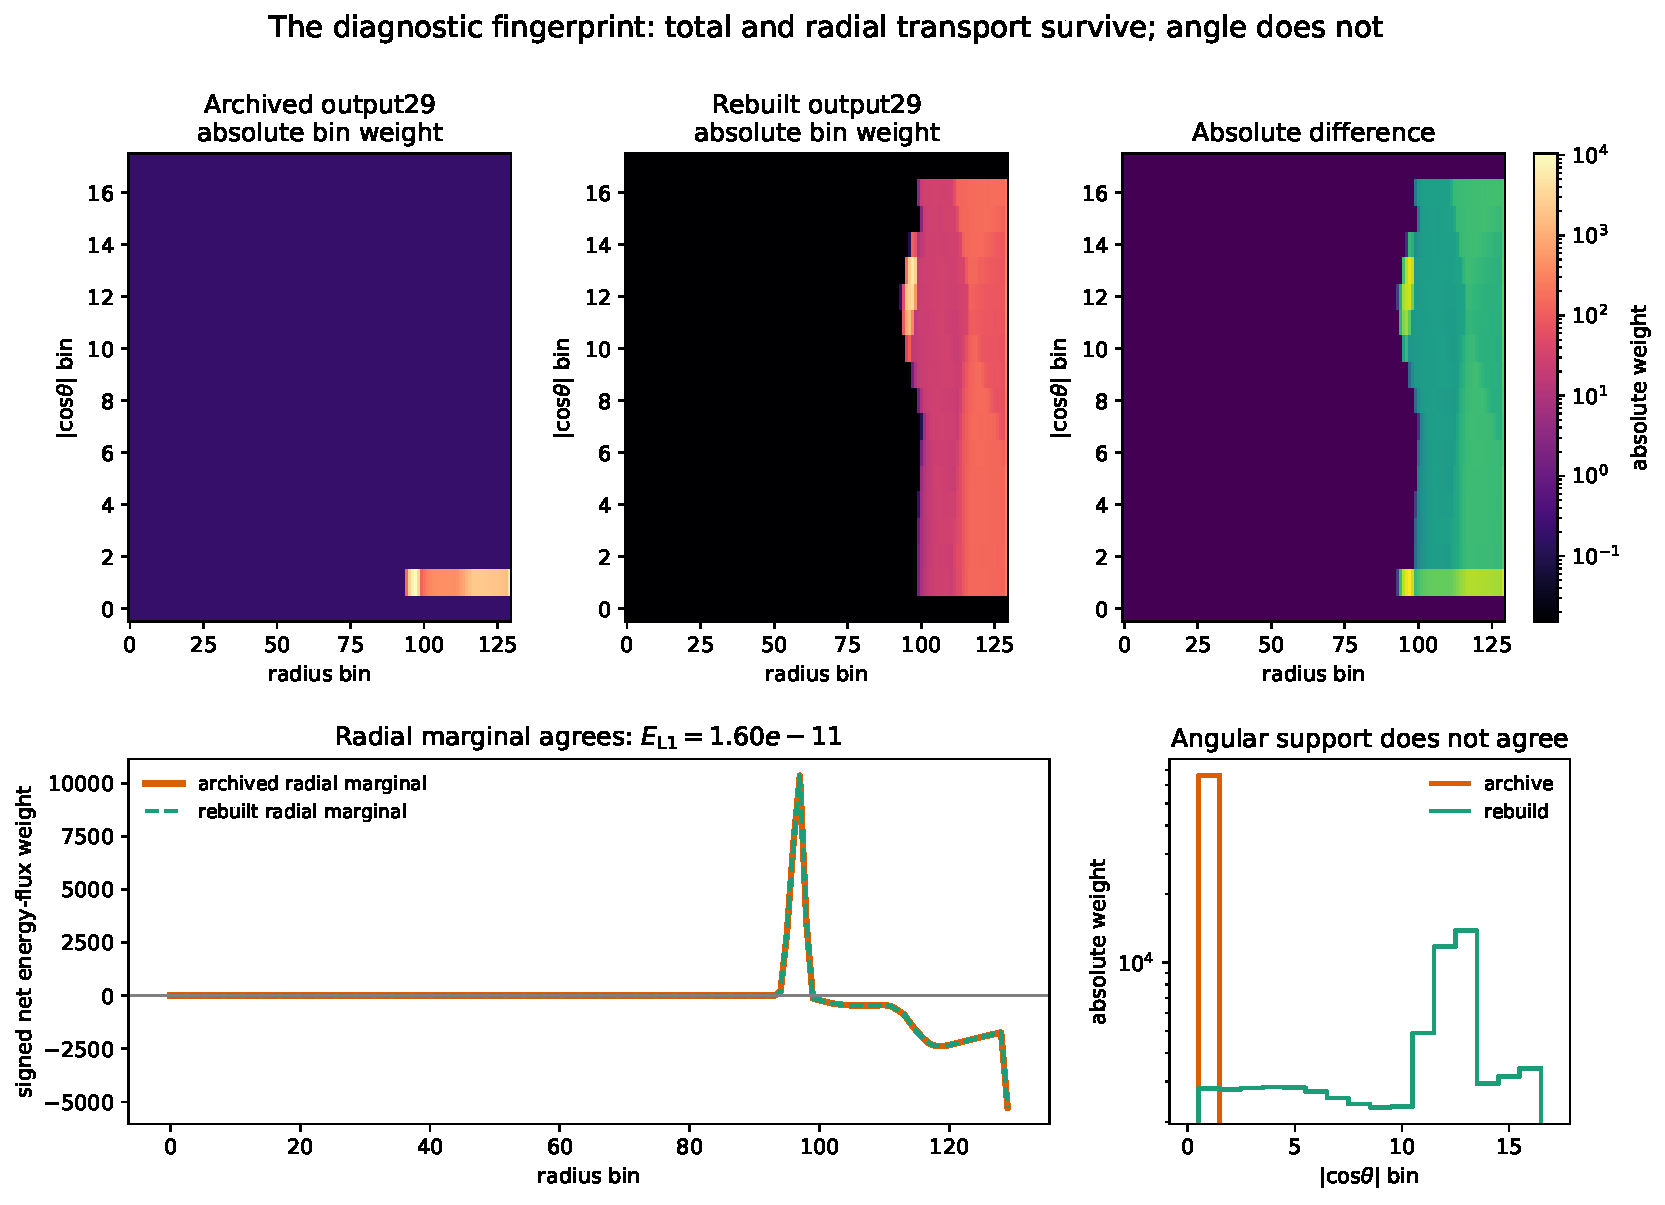
\includegraphics[width=\linewidth]{figures/output29_corruption_signature.pdf}
\caption{Eight-shard comparison at exact archived PDF time
\(10.520002963096713\). Inputs are the rebuilt dense \codeword{output29} and
the matching first eight archived sparse shards. Generated by
\artifact{docs/explanatory\_writeups/scripts/generate\_figures.py}.}
\end{figure}

\lookat Start with the lower-left panel. The archived and rebuilt radial curves
sit on top of each other. Now move to the lower-right panel: the absolute-weight
angular-support marginals separate sharply. The radial agreement tells us the
source state and radial accounting survived. The failure appears only when
angle matters.

\caveat This is an eight-shard matched-subset comparison, not a complete
1024-shard reconstruction. It tests the corruption signature and numerical
repair path. It does not certify global AMR completeness.

\begin{figure}[ht]
\centering
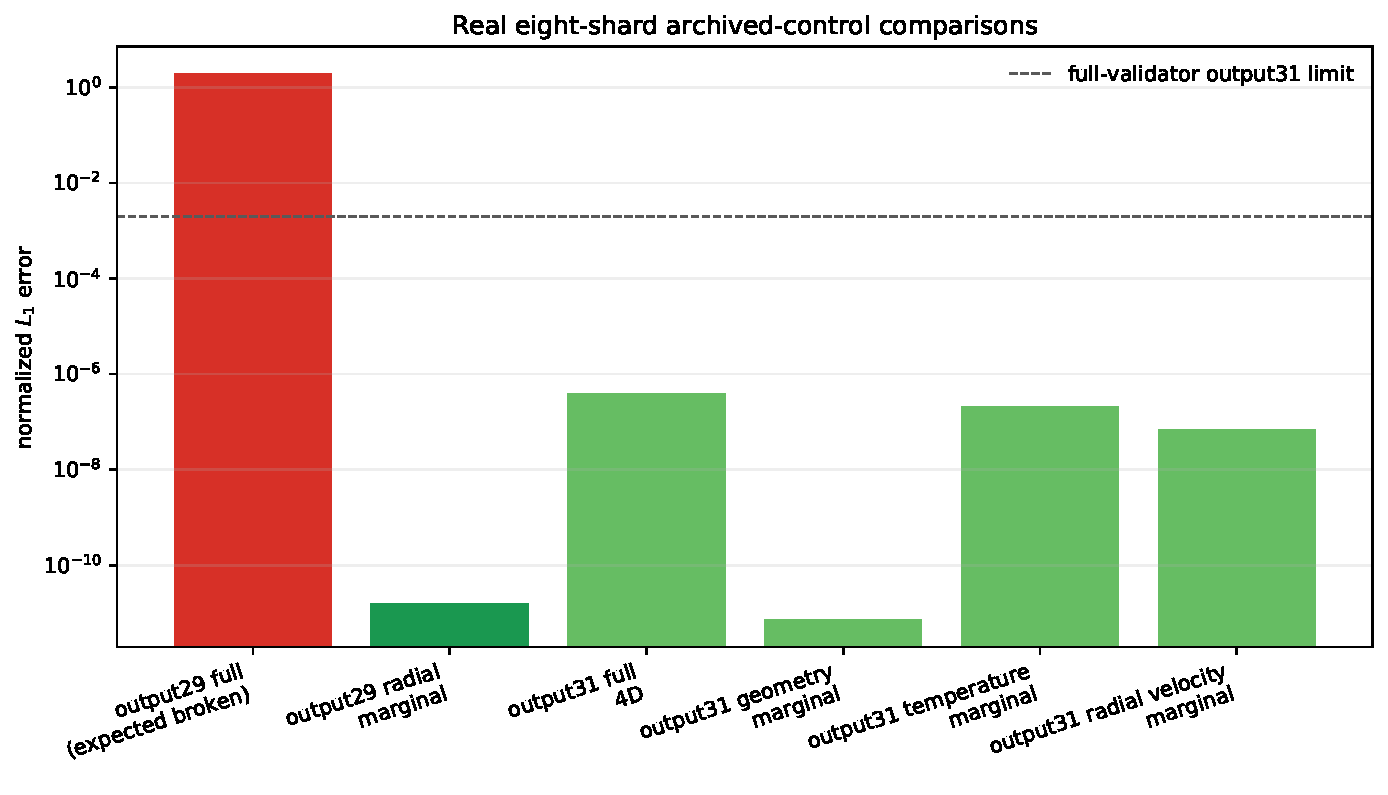
\includegraphics[width=0.96\linewidth]{figures/archived_control_errors.pdf}
\caption{Normalized \(L_1\) errors for the same eight-shard real-data
comparison. Green bars are quantities expected to survive the archive bug.
The red bar is the broken full archived \codeword{output29}.}
\end{figure}

\lookat The red bar is not a failure of the reconstruction. It is the required
negative control. A reducer that exactly reproduced the full archived
\codeword{output29} would have reproduced the broken angle. The green bars
show that the same reducer agrees closely with controls that should be intact.

\caveat The dashed \(2\times10^{-3}\) line is the full-\codeword{output31}
validator limit only. The other controls use tighter, product-specific limits.

\section{The key figures}

The cartoon explains the mechanism. The paired radial-and-angular comparison
is the evidence that makes it convincing. Exact inputs and metrics are recorded
in the root-level \codeword{figure\_metrics.json} ledger.

\section{What works}

This story earns confidence because it explains the exceptions, not just the
failures:
\begin{itemize}
  \item it identifies the exact source operation;
  \item it explains why twelve streams collapse in radius;
  \item it explains why \codeword{output29} has a salvageable radial marginal;
  \item it explains why \codeword{output31} is a useful negative control for
        this specific bug;
  \item it predicts the repaired-angle disagreement without requiring lost
        simulation state.
\end{itemize}

\section{What does not work}

The archive cannot be fixed by relabeling bins or renormalizing totals. Once a
joint coordinate was erased before binning, the missing association between
cell weight and angle is gone from that PDF file. The twelve broken streams
need reconstruction from the saved full-volume AMR outputs.

Also, ``all PDFs are broken'' is too strong. \codeword{output31} remains useful,
and the angle-integrated radial marginal of \codeword{output29} remains useful.
Those exceptions are part of the evidence, not inconvenient details.

\section{How this could be wrong}

A skeptical alternative would be a reader bug, a malformed sparse format, or
bad simulation state. Those alternatives do not explain why one marginal
survives while the joint distribution fails. Still, the source diff plus this
fingerprint is not a unique causal intervention: another angle-specific writer
bug could imitate part of the same result.
The production reader successfully reads the intact stream. The source state
reconstructs both intact controls and the preserved marginal. The source diff
contains an operation with exactly the expected destructive semantics.

The leading root cause is strong enough to guide the repair. The cleanest
remaining causal test is to run the same small AthenaK state with the bad line
present and absent and show that the mixed pattern appears and disappears.

\section{What would decide the issue}

For the existing archive, we know enough to act. To close the causal loop, run
a same-state bad-line/fixed-line A/B test with
\(n_{\rm mb}<n_{\rm mb,max}\). The regression must include both coordinate
orders, a trailing derived weight, and full-histogram comparison against an
oracle. Merely checking for nontrivial population can miss one of the two
reallocation paths. A post-write invariant that flags an unexpected \(100\%\)
underflow coordinate would catch the observed failure even earlier.

\section{Bottom line}

\bottomline The leading explanation is that one derived-coordinate calculation
reallocated shared coordinate storage twice in the mixed \codeword{output29}
case and once in the radius-first cases. The strongest evidence is not merely
the source diff. It is the source diff plus the peculiar fingerprint it
predicts: totals survive, one radial marginal survives, the angular joint
distribution fails, and the negative control remains intact. A same-state
old-line/new-line reproduction would upgrade this from strongly supported to
demonstrated.

\appendix
\section{Revision notes}

This document was revised after solution-advocate, logic/technical,
evidence/figure, red-team, visual-design, human-editor, and reproducibility
checks. Pass two added the second \(n_{\rm mb}\rightarrow n_{\rm mb,max}\)
reallocation, weakened the causal status pending an A/B writer test, separated
the eight-shard evidence from the incomplete archive-wide audit, and relabeled
\codeword{output31} as a differential negative control. Review records live in
the local \codeword{notes/} directory.

\end{document}
